% SPM8w.tex - Documentation for SPM8w r5236
% Heatherton & Kelley Labs
% Last update: March 2013 - DDW
%==========================================
%---Document Class
\documentclass[12pt]{article}

%---Load Packages
\usepackage[]{a4wide}   %Wider margins
\usepackage[]{times}    %Nicer fonts
\usepackage[usenames,dvipsnames]{xcolor} %color
\usepackage[]{currfile} %gets currfilename
\usepackage[]{lastpage} %Lastpage var
\usepackage[]{listings} %For inserting code
\usepackage[]{dirtree}  %For directory tree structures
\usepackage[]{graphicx} %For jpgs, needs pdftex on compile
\usepackage[]{hyperref} %For adding hyperlinks
\usepackage[]{minitoc}  %For section tocs

%---Additional Defintions
%--Extensions
\DeclareGraphicsExtensions{.pdf,.png,.jpg}
%--Colors
\definecolor{lightgrey}{rgb}{0.95,0.92,0.92}
\definecolor{dark-red}{rgb}{0.6,0.15,0.15}
\definecolor{dark-blue}{rgb}{0.15,0.15,0.4}
\definecolor{medium-blue}{rgb}{0,0,0.5}
%--Hyperlinks setup (removes boxes and changes link colors)
\hypersetup{colorlinks, linkcolor={dark-red}, citecolor={dark-blue},urlcolor={medium-blue}}
%=Code boxes setup (adjust frame and colors etc.)
\lstset{numbers=left, stepnumber=1, numbersep=5pt, numberstyle=\footnotesize\color{black},
basicstyle=\ttfamily\footnotesize, keywordstyle=\color{black}, commentstyle=\color{red},  stringstyle=\color{black}, frame=single, tabsize=4, backgroundcolor=\color{lightgrey},
breaklines=True}
%Make a command for horizontal rules. 
\newcommand{\HRule}{\par\noindent\color{orange}{\rule{\linewidth}{1mm}}}

%---Begin Document
\begin{document}
\dosecttoc %init minitoc for sections

%---Title Page
\begin{titlepage}
\begin{flushleft}
\vspace*{5cm}
\Huge SPM8w \\[-20pt]
\HRule 
\end{flushleft}
\vfill
\emph{SPM8w:} r5236 \\
\emph{LaTeX File:} \currfilename \vspace{-24pt}
\begin{flushright}
\today
\end{flushright}
\end{titlepage}

%---Table of Contents
\tableofcontents
\newpage

%===Start Manual
%=Section 1
\section{Downloading and Installing SPM8w}
\secttoc  %Inserts a minitoc
\subsection{Downloading SPM8w from github}
As of 2013, SPM8w has moved to github:\url{http://github.com/ddwagner/SPM8w} with the idea that this will make it easier for people to obtain the latest version (or revert to an older one) as well as to make it easier for people to commit changes or fixes to the code. As a result of this move to github, only elements of the code that I have permission to share will be found in the repository (i.e., elements of the core spm8 code and our edit of art\_repair). 

In order to install spm8w it is highly recommended that you, or someone in your lab, become minimally familiar with git and clone the spm8w repository using the following address: \textbf{https://github.com/ddwagner/SPM8w.git} and a local version of Git (available at: \url{http://help.github.com/articles/set-up-git}). Alternatively, if you do not want to use Git, you can go to the github address listed above and download a zip archive of the entire repository. 

\subsubsection{Why Git?}
\begin{figure}[ht]
\centering
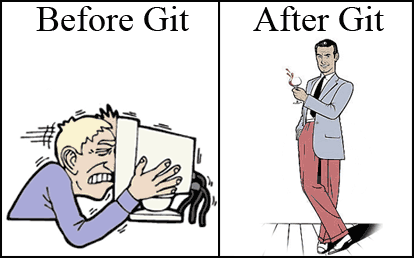
\includegraphics[scale=0.5]{./assets/1_git}
\end{figure}

One of the main advantages of using Git is that it will make it easy to retrieve small fixes to the current version of SPM8w as well as update to new versions as they become available on the github repository. In addition, it opens up the possibility of creating separate branches, so that newer versions can coexist alongside older ones allowing you to run new studies with the latest SPM8w version but still be able to go back and work with older versions. Finally, it will make it easier to engage in collaborative coding, that is to say that anyone can contribute changes or fixes and these will eventually be merged into the main branch. 

\subsubsection{Installing SPM8w with Git}
The following is a brief description of how to clone SPM8w repository using Git and how to check for updates. It is highly recommended that you take a look at one of the many brief introductions to Git prior to running these commands, for instance the "simple guide - no deep shit!" web page is a great place to start  \url{ http://rogerdudler.github.com/git-guide/}

Cloning the SPM8w repository using git is extremely easy. Once git is installed on your system, open a terminal window on linux/mac or Git Bash on Windows and navigate to the directory you want to install SPM8w. For instance, your MATLAB directory on your local computer. From within that directory enter the following command:

\begin{lstlisting}
$ git clone git://github.com/ddwagner/SPM8w.git
\end{lstlisting}

Git will proceed to clone the SPM8w repository, this includes not only the core spm8w files, but also some nifti files used by SPM8w as well as files to help configure the matlab path (under the MATLAB directory). In addition, you will find a PDF directory that contains the latex file that was used to build this PDF and a copy of this PDF.  

\subsubsection{Updating SPM8w}
Currently there is only one branch of SPM8w on github, this is the master branch that I am currently working from. Once this version is finalized and tested (sometime in February 2013), I will create a development branch for myself and anyone else to work on. 

What this means for people who use SPM8w is that you can pull or clone this finalized, hopefully stable, branch and need not worry about current development introducing new bugs. Although development on this master branch will cease, small bug fixes will be incorporated. In order to easily update these fixes into your current SPM8w build you can simply use the Git pull command to sync your files with the latest on github. [note: once I have a better sense of how the branching will work, I'll update this section with details on how to select which branch to clone]. 
  
\begin{lstlisting}
$ git pull
\end{lstlisting} 

\subsection{Setting up the matlab paths}
Inside the MATLAB directory that comes with SPM8w is a file called \textbf{spm8path.m}  which you can use to help you set up your matlab path for use with SPM8/SPM8w and other commonly used matlab-based tools for neuroimaging. In order to use this file, you will need to edit the following lines in order to specify the path to SPM8 and to SPM8w. 

\lstinputlisting[language=Matlab, firstline=21, lastline=23]{../ADDITIONAL_FILES/SPM8path.m}

In addition, if you installed tools (\emph{see next section}) to the TOOLS directory of SPM8w, you can add this directory to the tools\_path variable as well as the name of the tools in subsequent variables (comment out any that you do not use). 

\lstinputlisting[language=Matlab, firstline=25, lastline=33]{../ADDITIONAL_FILES/SPM8path.m}

In order to use \textbf{spm8path.m} to set your path you can either place it inside your default matlab path directory and call it from the matlab command prompt or create a bash script that tells matlab to run \textbf{spm8path.m} upon starting.
\begin{lstlisting}
$ matlab -r spm8path.m
\end{lstlisting}

\subsection{Microsoft Windows compatibility}
In general, SPM8w is compatible with Windows. However, as many of the functions are developed on Linux first, the newer functions may not have been fully tested with Windows. Whenever possible SPM8 uses matlab commands to perform OS level operations (i.e. chdir, move, copy and delete files). In a few cases, it is necessary to rely on system commands, for that purposes SPM8w will call spm8w\_osbabel.m, a tool written to translate the default Linux commands into their windows equivalent. However this is slowly being depreciated as I only recently realized that pretty much every system command that SPM8w needs, has a cross-platform matlab equivalent. 

SPM8w r5236 has been tested in a virtual machine of Windows XP running MatlabR2010b. So far results are identical to those run on Linux. However, owing to differences in how the Matlab command window works, some of the text output to the command window is poorly formatted due to no text wrapping. This is relatively rare and constitutes a minor cosmetic inconvenience. This is also true of Linux unless running the Matlab interpreter in a terminal which is what SPM8w's command window output was optimized for. 

\subsection{Example Dataset and additional files}
The easiest way to learn how to use SPM8w and to ensure that your local version is working is the run through an example dataset. SPM8w comes with a short dataset of a fictional study called \textbf{H8TJAZZ} (if you really need to know where that title comes from, \href{http://www.youtube.com/watch?v=bKwQ_zeRwEs}{click here}). This example dataset comes with all the different Parameter files needed to run most analyses that SPM8w is capable of and can be used to build Parameter files for running your own studies.

SPM8w also comes with additional high-quality anatomical MRIs in MNI space that are of higher resolution than the files that come with SPM8. These files can be found in the \textbf{ADDITIONAL\_FILES} directory in your local repository. The files in the canonical.7z archive should be extracted and placed inside the canonical directory of your local SPM8 copy. 

\subsection{Additional requirements}
As we will see further in the following sections, SPM8w is nothing more than a series of scripts to interface with various components of SPM8. As such it requires a working installation of SPM8 to reside in the matlab path. Moreover, each version of SPM8w requires a specific revision of SPM8 to work correctly. This is largely due to the fact that we duplicate a number of core SPM8 files and make some small edits to them (in most cases simply removing graphics and increasing details of the output). To make things simple, SPM8w versions are named after their associated SPM8 revision. Thus, the current version of SPM8w (\emph{r5236}) requires SPM8 r5236 (\url{http://www.fil.ion.ucl.ac.uk/spm/software/spm8/})

SPM8 can also benefit from additional toolboxes. Here is a list of toolboxes we typically use in our environment, although none are required for SPM8w to function.
 
\begin{description}
\item[Anatomy Toolbox 1.8] \hfill \\ 
\href{http://www.fz-juelich.de/SharedDocs/Downloads/INM/INM-1/DE/Toolbox/Toolbox_18.html}{http://www.fz-juelich.de/.../INM/INM-1/DE/Toolbox/Toolbox\_18.html}
\item[Marsbar 0.43] \hfill \\ 
\href{http://marsbar.sourceforge.net/}{http://marsbar.sourceforge.net/}
\item[WFU Pickatlas 3.0.3, requires Matlab 7.6 or better] \hfill \\ \href{http://fmri.wfubmc.edu/software/PickAtlas}{http://fmri.wfubmc.edu/software/PickAtlas}
\item[WFU Pickatlas 2.5.2, for Matlab 7.4] \hfill \\ \href{http://fmri.wfubmc.edu/software/PickAtlas}{http://fmri.wfubmc.edu/software/PickAtlas}
\item[BredeQueury 2009/03/12] \hfill \\ 
\href{http://www2.imm.dtu.dk/pubdb/views/publication_details.php?id=5706}{http://www2.imm.dtu.dk/pubdb/views/publication\_details.php?id=5706}
\item[Automated Labeling Toolbox (SPM8 version)] \hfill \\ \href{http://www.cyceron.fr/web/aal__anatomical_automatic_labeling.html}{http://www.cyceron.fr/web/aal\_\_anatomical\_automatic\_labeling.html}
\item[VBM 8 r435 (December 2011)] \hfill \\ 
\href{http://dbm.neuro.uni-jena.de/vbm/download/}{http://dbm.neuro.uni-jena.de/vbm/download/}
\end{description}

In addition, there are also a number of stand alone tools that are typically part of our environment that you may find handy. Once you download these, you can choose to install them into a TOOLS directory and edit the \textbf{spm8path.m} (\emph{see Section 1.2}) to reflect the location of these tools. 
 
\begin{description}
\item[XJVIEW 8.9 - modified, see below] \hfill \\ \href{http://www.alivelearn.net/xjview8/xjview.m}{http://www.alivelearn.net/xjview8/xjview.m} \\ \href{http://www.alivelearn.net/xjview8/Tdatabase.mat}{http://www.alivelearn.net/xjview8/Tdatabase.mat}
\item[CONN (Connectivity Toolbox)] \hfill \\ \href{http://www.nitrc.org/projects/conn/}{http://www.nitrc.org/projects/conn/}
\item[r2a\_GUI 2.7] \hfill \\ \href{http://r2agui.sourceforge.net/}{http://r2agui.sourceforge.net/}
\item[GLM\_Flex (for running mixed ANOVAs with 3+ factors)] \hfill \\ \href{http://nmr.mgh.harvard.edu/harvardagingbrain/People/AaronSchultz/GLM_Flex.html}{http://nmr.mgh.harvard.edu/.../People/AaronSchultz/GLM\_Flex.html}
\item[SNPM8b] \hfill \\ \href{http://www2.warwick.ac.uk/fac/sci/statistics/staff/academic-research/nichols/software/snpm/}{http://www2.warwick.ac.uk/.../academic-research/nichols/software/snpm/}
\end{description}

Note that XJVIEW expects the AAL, Brodmann and ch2 volumes (see the \\ \textbf{ADDITIONAL\_FILES} directory mentioned above) to be in img/hdr format whereas ours are in NIFTI. Thus the file xjview.m needs to be modified (around lines ~3700) to change the extensions to .nii. Any upgrades to newer versions will need to be edited as well.
\newpage

%=Section 2
\section{Preparing a study for SPM8w}
\secttoc %Inserts a minitoc
\subsection{Study Directory Structure}
SPM8w requires that your data conform to its expectations regarding naming and directory conventions. Although some flexibility in subject and directory naming is allowed, by and large it is highly recommended that users conform to the standard layout for a study analyzed in SPM8w. This can be considered the main disadvantage of using SPM8w as it forces the user to buy into its way of organizing files. Users taunting SPM8w with idiosyncratic directory and file names do so at their own peril. 
\vspace{\baselineskip}

\noindent The following is a minimal example of a new study ready to be processed with SPM8w (Note that these specifications have been changed as of SPM8w r5236):
\vspace{\baselineskip}
\dirtree{%
.1 /H8TJAZZ.\DTcomment{Name of the study directory}.
.2 ONSETS.\DTcomment{Where onsets for GLM models are stored}.
.3 H8TJAZZ\_BLOCK.\DTcomment{Where onsets for a Block design GLM are stored}.
.3 H8TJAZZ\_ER.\DTcomment{Where onsets for a rapid ER design GLM are stored}.
.2 SCRIPTS.\DTcomment{Where parameter files for spm8w are stored}.
.2 SUBJECTS.\DTcomment{Where all subject files are stored}.
.3 01jan13aa.\DTcomment{Directory name for a single subject}.
.4 NIFTI.\DTcomment{NIFTI dir containing clean gziped NIFTI files}.
.3 01jan13bb.
.4 NIFTI.
.3 RAW.\DTcomment{Directory containing all raw subject files}. 
}
\vspace{\baselineskip}
In order to begin using SPM8w, it is necessary to set up a directory structure as in the above. One way to make that easier is to copy the example dataset to a new directory and replace its files with your own. In addition you can discard any parameter files you won't need (VOI, ROI etc.) and then rename and edit the example parameter files to conform to your study specifications. 

It is worth pointing out that the above directory structure requires that the un-preprocessed NIFTI files for each subject exist in a NIFTI directory within that subjects directory. The reason for this is two-fold. First, SPM8 will write various spatial transformations to the NIFTI header of each file, thus making it difficult to start an analysis or preprocessing over from scratch. This can be problematic if attempting to normalize using DARTEL and then going back and deciding instead to use the EPI template as the files now contain transformations specific to DARTEL preprocessing. The second reason for this convention is that re-analyzing from scratch becomes simply a matter of deleting all the files in a subject's directory and making new copies of the unpreprocessed NIFTI files. This ensures that no files are leftover from the previous analysis. 

In addition, SPM8w expects, but does not require, a RAW directory containing the raw scanner specific files (e.g., Philips PAR/REC). If raw files are already in NIFTI, then the RAW directory is unnecessary and need not be created. The main reason for the RAW directory is to ensure that all the files needed for an analysis are within the study directory. In this way a full archive of the study upon completion becomes simply a matter of making a copy of the study root directory. 

During various stages of analysis, SPM8w will create new directories for storing the output of different operations. A fair amount of work has gone into keeping things organized and avoiding file collisions. Below is an example of the directory structure of a study that has gone through a number of stages of analysis (e.g., preprocessing, 1st and 2nd level GLMs, PPI analysis, Resting state analysis and ROI analysis):
\vspace{\baselineskip}
\dirtree{%
.1 /H8TJAZZ.
.2 ONSETS.
.3 H8TJAZZ\_BLOCK.
.3 H8TJAZZ\_ER.
.2 RFX.\DTcomment{Where 2nd Level GLMs are stored}.
.3 RFX\_H8TJAZZ\_BLOCK.\DTcomment{A 2nd level RFX analysis}.
.3 RFX\_H8TJAZZ\_ER.\DTcomment{Another 2nd level RFX analysis}.
.2 ROI.\DTcomment{Directory where results of ROI analyses are stored}.
.3 ROI\_images.\DTcomment{Directory containing anatomical ROIs}.
.3 ROI\_H8TJAZZ\_BLOCK.\DTcomment{Results of ROI analysis for a 2nd level GLM}.
.2 SCRIPTS.
.2 SNR\_BOLD.\DTcomment{Results of SNR calculation on BOLD timeseries}.
.2 SNR\_REST.\DTcomment{Results of SNR calcualtion on REST data}.
.2 SUBJECTS.
.3 01jan13aa.
.4 ANATOMY.\DTcomment{Where anatomical files are stored}.
.4 FUNCTIONAL\_BOLD.\DTcomment{Where functional data are stored}.
.4 NIFTI.
.4 REST.\DTcomment{Where resting state data are stored}.
.4 RESULTS.\DTcomment{Where all 1st level GLM results are stored}.
.5 GLM\_H8TJAZZ\_BLOCK.\DTcomment{A 1st level GLM}.
.5 GLM\_H8TJAZZ\_ER.\DTcomment{Another 1st level GLM}. 
.3 01jan13bb.
.4 ANATOMY.
.4 FUNCTIONAL.
.4 NIFTI.
.4 REST.
.4 RESULTS.
.5 GLM\_H8TJAZZ\_BLOCK.
.5 GLM\_H8TJAZZ\_ER.
.3 DARTEL.\DTcomment{Where DARTEL study-wise templates are stored}.
.3 RAW.
}

\subsection{Data formats and conversion of prior studies}
SPM8w has been written to work exclusively with uncompressed NFITI files, although some components do still read/write to NIFTI formatted img/hdr files. By and large, SPM8w will no longer accept 3D img/hdr files as input and expects only 4D NIFTI files. 

Within Dartmouth using the Philips Intera MRI scanner, it is advisable that data be exported direct to NIFTI from the scanner console and that these NIFTI files be used as input to SPM8w. However, it is often the case that only raw data (i.e., Philips PAR/REC files at Dartmouth) are available. In this case, there are a number of ways to convert PAR/REC files to NIFTI, each with varying degrees of abject failure. At the moment, the best solution in terms of getting it "right" appears to be the matlab based r2a\_gui tool (\emph{see next section}). Other PAR/REC converters either make mistakes or are incompatible with older (or newer) versions of the PAR/REC format. 

Occasionally, people have older studies analyzed with our older set of scripts (i.e., \\spm2\_analyse) that they would like to re-analyze with SPM8w. Rather than convert from scratch it is possible to convert the img/hdr files to NIFTI. However, it is important to understand that since the img/hdr files kept none of the original transformations that are typically preserved with NIFTI (i.e., \emph{sform} and \emph{qform} fields), these converted NIFTI files will also have no transformations and the origin will be set to the center of the volume. In practice, this has seldom been a problem as many people typically normalize to the EPI template. Moreover, if good registration between MRI and EPIs are needed then SPM's coregistration function is generally able to provide the appropriate transformation. However, given the loss of header information this is no longer advised and it is recommended that you always begin from raw data. 

\subsection{PAR/REC Converter}
The current favorite converter for converting raw PAR/REC files to NIFTI is the matlab based converter r2a\_gui (available here: \url{http://r2agui.sourceforge.net/}). Across multiples years of our Philips data, this has been the converter that appears to do the best job in maintaining appropriate header fields and works well for creating nifti files that are compatible with  SPM, AFNI and FSL. 

The downside to using this converter is the gui itself. In order to get around it and to ensure the output of this converter conforms to our directory and file naming specifications, SPM8w comes with a matlab script (spm8w\_nifticonverter.m) that runs r2a\_gui renaming and moving the converted files to their appropriate place.  

In order to use spm8w\_nifticonverter.m you must have your raw PAR/REC data stored in a compressed tar archive of the same name as the subjectID (raw\_01feb13aa.tar.gz). This archive should contain a single directory (also of the same name as the subjectID) which itself contains the raw PAR/REC files (the names of which can be anything). To make it easy to make such archives, SPM8w comes with a script (spm8w\_rawtar.m) that use crossplatform matlab commands to create compressed tar archives from directories containing raw files for a single subject. Once again, it is important that these directories be of the same name as your subject ID as this is how SPM8w determines subject names. 

For instance, if you have a directory with the following:
\vspace{\baselineskip}
\dirtree{%
.1 /01feb13aa.
.2 01feb13aa\_03\_1-FEEPI.PAR.
.2 01feb13aa\_03\_1-FEEPI.REC.
.2 01feb13aa\_04\_1-FEEPI.PAR.
.2 01feb13aa\_04\_1-FEEPI.REC.
}
\vspace{\baselineskip}
You can use spm8w\_rawtar to create a compressed tar archive using the following command: 
\begin{lstlisting}
$ spm8w_rawtar('01feb13aa')
\end{lstlisting}

To select multiple directories you can call spm8w\_rawtar without arguments and a window will appear allowing you to make multiple selections. Afterwards, move these subjID.tar.gz files to your study's raw directory (i.e., H8TJAZZ/SUBJECTS/RAW). Then run spm8w\_nifticonverter from the study root directory either by using button in the SPM8w gui or by calling it directly from the matlab prompt. 
\newpage

%=Section 3
\section{Parameter Files}
\secttoc  %Inserts a minitoc
\vspace{\baselineskip}
Almost every function in SPM8w is script driven according to the parameters specified in the various parameter file types (P,R,CON,ROI,VOI) which exist in the SCRIPTS directory. Notwithstanding the ease of running complex analyses, relying on simple scripts (m-files) also ensures that a full record is kept for each study's analysis pipeline. Thus, with the right version of SPM and SPM8w, an entire analysis can be recreated from Raw data to final results from the Parameter files alone. Many SPM functions rely on a consistent naming for parameter files and use filters to search for them. Thus it is important that the naming conventions for parameter files are followed. 

\subsection{The P file}
The P parameter is the workhouse of SPM8w and controls everything from preprocessing (both functional and anatomical) to GLM estimation and cluster based correction (using AFNI's alphasim).  
For a single study, it is quite common to have more than one P file. One of which specifies the preprocessing steps (which is typically done once) and multiple P files for different GLM models. Below, we walk through the various sections of the P file from the example dataset. 

In this section, the path to the study directory and directory names for the RAW, GLM and RFX directories are set (all relative to the study\_dir). In addition, you can optionally specify the CON you intend to use with this P file. Doing so will save you from having to select it later and allow you to spend more time drinking gin \& tonics by the department pool. If you would rather always select the CON file, simply comment out this line. 

\lstinputlisting[language=Matlab, firstline=7, lastline=12]{../EXAMPLE_DATA/2013_H8TJAZZ_SPM8w_r5236/SCRIPTS/P_H8TJAZZ.m}
Here, the onset specifications are set, including the directory in which the onsets are stored (relative to STUDY/ONSETS) and any prefix or extensions that are required. Using this scheme it is possible, for instance, to have subject specific onsets, subject specific durations or subject specific parametric modulators as well as a combination of these (i.e., everyone has the same onsets, but different duration and parametric modulators).
 
\lstinputlisting[language=Matlab, firstline=14, lastline=19]{../EXAMPLE_DATA/2013_H8TJAZZ_SPM8w_r5236/SCRIPTS/P_H8TJAZZ.m}
Here is where the condition type and labels are set. SPM will use the condition names to find the onsets based on the onset specifications. Simply put, SPM8w will look in the H8TJAZZ/ON\-SETS/H8TJAZZ directory for files called human.txt, animal.txt, vegetable.txt and mineral.txt. If the onsets prefix had been set to [p.subj,'\_'] then SPM8w would now look for files called 01feb13aa\_human.txt, 01feb13aa\_animal.txt, etc. etc. For examples on block (p.block\_cond) and regressor only designs (p.reg\_cond) see the example dataset. 

\lstinputlisting[language=Matlab, firstline=21, lastline=24]{../EXAMPLE_DATA/2013_H8TJAZZ_SPM8w_r5236/SCRIPTS/P_H8TJAZZ.m}
In this section, scanning parameters are specified. In addition, it is possible to have a different number of TRs per session. For instance, in 3 sessions of data where run 1 and 3 are identical but run 2 was longer, the p.nTR would be specified like this:
\begin{lstlisting}
p.nTR = [120,250,120];
\end{lstlisting}

\lstinputlisting[language=Matlab, firstline=26, lastline=30]{../EXAMPLE_DATA/2013_H8TJAZZ_SPM8w_r5236/SCRIPTS/P_H8TJAZZ.m}
The following section sets the preprocessing and related quality assurance routines. Many of these are self-explanatory, however it is worth nothing that p.snr will calcularte voxel-wise snr, sd and average volumes and place these in the H8TJAZZ/SNR\_BOLD folder. p.slices calculates slice-wise noise (using components of slices\_analyse from Antonia Hamilton: \url{http://dbic.dartmouth.edu/wiki/index.php/Noise_Detection}).

\lstinputlisting[language=Matlab, firstline=32, lastline=42]{../EXAMPLE_DATA/2013_H8TJAZZ_SPM8w_r5236/SCRIPTS/P_H8TJAZZ.m}
This following section describes the specifications for the GLM analysis.

\begin{description}
\item[p.normtype:] Specifies which normalization files serve as input to GLM computation. Setting normtype to OLD will use files normalized with the EPI template. Setting normtype to DARTEL will use files normalized with dartel and VBM8 (not entirely supported yet) will use files normalized with DARTEL using VBM8's templates. The advantage of this parameter is it allows for both Dartel and EPI template based normalization files and analyses to co-exist.
\item[include\_run:] This setting determines which run (i.e., session) will be modeled. Options are 'all' for all sessions. A single number for only one run (e.g., p.include\_run = 2;) or a vector of runs (.e.g, p.include\_run = [1,3];)
\item[p.polyord:] Number of polynomials to detrend with. Typically we use p.polyord = 1 which is equivalent to a linear trend + constant (i.e., our old linear trend regressor in prior versions of SPM8w). However it is possible to include more polynomials, which may be useful for detrending longer runs.
\item[p.move:] Enables or disables inclusion of motion regressors. Under cases of very small motion, it may be advisable to not model motion at all.
\item[p.outliers:] Enables inclusion of dummy regressors for outlier volumes as calculated by art-\_detect (run using spm8w\_art.m). There is no harm to leaving this on, as if no files detailing which scans are outliers are found, then GLM computation will proceed. In this way it's possibly to only model outliers for subjects who have files describing which scans are outliers.
\item[p.demean:] Optional setting to demean task regressors prior to GLM computation. This was the default behavior in SPM99 but, as far as I can tell, was accidentally left out of SPM2 and never repaired as it has no effect on beta estimates. Will Penny from the spm list: \textit{"SPM2 doesn’t mean centre regressors whereas SPM99 did. It is an inconsistency but not one of great import as it will have no effect on the parameter estimates or resulting inference (it will change the estimate of the constant term but nothing else)."} It does, however, result in SPM orthogonality checks which are difficult to interpret. Turning this on should have no effect on results, but make SPM's default orthogonality check easier to interpret.
\item[p.durtime:] Durations are expressed in seconds or TRs. If durations are in seconds (e.g. reaction times), SPM8w will convert them to TRs. This works for block and event-related designs but if you use this all durations must be in seconds (e.g. both the states and items in a state-item design). Spm8w will always warn you during estimation if it divides by TR.
\item[p.disable\_orth:] SPM's within trial type orthogonalization is disabled. SPM defaults to orthogonalizing within trial regressors (i.e., successive parametric regressors or successive FIR regressors). This option allows you to disable this behavior. At present it strikes us as undesirable to orthogonalize FIR regressors. Importantly, this variable expects that you have replaced the stock spm\_fMRI\_design.m file with the modified spm\_fMRI\_design.m file that can be found in SPM8w's ADDITIONAL\_FILES directory. 
\end{description}

\lstinputlisting[language=Matlab, firstline=44, lastline=52]{../EXAMPLE_DATA/2013_H8TJAZZ_SPM8w_r5236/SCRIPTS/P_H8TJAZZ.m}
The following section pertains to DARTEL normalization. In general the defaults provided here are likely to be best. If you intend to use DARTEL based normalization on EPI data it is imperative that you coregister your anatomical to your EPI (p.coreg2epi = 1). 

\lstinputlisting[language=Matlab, firstline=54, lastline=66]{../EXAMPLE_DATA/2013_H8TJAZZ_SPM8w_r5236/SCRIPTS/P_H8TJAZZ.m}
Optional specifications for running Monte Carlo simulations using spm8w\_alphasim.m, a matlab wrapper for AFNI’s AlphaSim program. To use this function requires that you have a local version of AFNI in your path (see tools section below for more information on spm8w\_alphasim.m).

\lstinputlisting[language=Matlab, firstline=73, lastline=80]{../EXAMPLE_DATA/2013_H8TJAZZ_SPM8w_r5236/SCRIPTS/P_H8TJAZZ.m}
The following section details some of the advanced settings for HRF modeling, filtering and realignment. 

\begin{description}
\item[p.hrf:] Specifies which model of the HRF to use. 
\item[p.hrfwindow:] For FIR designs: Duration (window) of modeled HRF. Needs to be approximately 20 seconds to capture the full HRF. 
\item[p.hrfbasis:] For FIR designs: Number of basis sets with which to model the HRF. Should be an integer (preferably p.hrfwindow / TR). So for a 20 second window, with a TR of 2.5, p.hrfbasis would be 8 (i.e. 8 time bins of 2.5s). 
\item[p.hpf and p.autocorr:] Additional options include high pass filtering and serial autocorrelation correction. These should only be used if you have a single run of data and are feeling adventurous. Although, according to Darren Gitelmen at an MGH workshop, it is not quite a cardinal sin to run HPF and autorcorrelation correction on concatenated runs, but nevertheless this has not been our convention. 
\item[p.refslice and p.realign\_rtm:] Specifies which slice to use as reference slice for slicetime correction and whether realignment should take place relative to the 1st slice (1pass) or if realignment should use a 2pass solution realigning to the 1st run then to the session mean. In general we always use slice 1, but this can vary depending on acquisition sequence.
\item[p.overridedel:] If set to 0, SPM8w will always ask if you wish to delete prior analyses before overwriting them (i.e., when redoing preprocessing or GLM computation). The reasoning for this setting is to ensure that analysis directories remain free of clutter from prior analyses, SPM8w will typically delete the entire FUNCTIONAL directory (saving only outlier files) and check out fresh copies from the NIFTI directory. If you decide to store your diary and personal photographs inside a subject's FUNCTIONAL or ANATOMICAL directory, you will lose them. p.overridedel = 0 will cause SPM8w to ask you for confirmation prior to deleting prior data directories. Although, this may seem desirable it requires you to answer this question for every subject. 
\end{description}

\lstinputlisting[language=Matlab, firstline=82, lastline=100]{../EXAMPLE_DATA/2013_H8TJAZZ_SPM8w_r5236/SCRIPTS/P_H8TJAZZ.m}
There are some additionally settings in the P file no discussed here. To find out more, read the comments in the P files provided with the example dataset. 

\subsection{The R file}
The R file is the resting state equivalent to the P file, but is still very much a work in progress (this section is just a placeholder). 

\subsection{The CON file}
The study contrasts file specifies the type of contrast to perform on the conditions from the GLM. Contrasts are zero padded to fill in nuisance regressors. This is especially useful in situations where the number of regressors in the model differs per subject (e.g. if p.outliers = 1) or for mixed designs and FIR models where the number of regressors can easily reach 100 (see CON\_H8TJAZZ\_MIXED.m for an example of some tricks for making organized contrast vectors for a state-item study). The way this works is that SPM8w will searche through the regressor names and count the number of 'r' regressors (which is the name we reserve for nuisance regressors). It is therefore important to keep in mind that this 'trick' will fail if you hack in any custom nuisance regressors and don’t name them 'r'. If you let SPM8w make the nuisance regressors for you, then this should always be correct. 

Protip: ensure that your contrast vectors always sum to zero (except for vs. baseline) and that your contrast weights never exceed one. For instance, [3 -1 -1 -1] while a valid contrast that will generate an appropriate statistical map, the underlying beta values are multiplied by the contrast weights. Thus, when you go to extract con values for an ROI analysis, the values will be scaled by the weights. All statistics on such values will be valid, but when you go to plot the results, the y-axis may appear to be overly large! 

\lstinputlisting[language=Matlab, firstline=7, lastline=17]{../EXAMPLE_DATA/2013_H8TJAZZ_SPM8w_r5236/SCRIPTS/CON_H8TJAZZ.m}
\lstinputlisting[language=Matlab, firstline=19, lastline=28]{../EXAMPLE_DATA/2013_H8TJAZZ_SPM8w_r5236/SCRIPTS/CON_H8TJAZZ.m}

\subsection{The ROI file}
The ROI parameters file specifies the parameters for ROI analyses. Everything from the creation of  ROIs, to the extraction of parameter estimates, and finally to summary statistics (descriptives, t-tests, correlations) is controlled from the parameters in this file.  

The following section of the ROI parameter file specifies where the ROI analysis results will be written (roi\_dir) which RFX directory contains the con images (rfx\_dir). The optional location of the directory containing a priori ROIs (i.e., anatomical or some other source; roi\_img\_dir). And finally the filename of excel spreadsheet files containing roi specifications and subject variables (see the xlsx files provided with the example dataset to understand the layout). Note that the roi\_spec\_file is optional. ROI specifications can also be defined in a variable (see below) and will be used if the roi\_spec\_file does not exist.

\lstinputlisting[language=Matlab, firstline=7, lastline=13]{../EXAMPLE_DATA/2013_H8TJAZZ_SPM8w_r5236/SCRIPTS/ROI_H8TJAZZ.m}
This section describes the conditions from which the parameter estimates will be extracted. These conditions must match those in the CON parameter file that is associated with this particular RFX analysis. Put differently, spm8w\_roitool.m will extract parameter estimates from files in the RFX/RFX\_H8TJAZZ/humVSbas directory (and so forth). 

\lstinputlisting[language=Matlab, firstline=16, lastline=23]{../EXAMPLE_DATA/2013_H8TJAZZ_SPM8w_r5236/SCRIPTS/ROI_H8TJAZZ.m}
This section defines the roi specs requiring a region name, an MNI coordinate and a size in mm's (for spherical ROIs). If a filename is provided instead of an ROI size then spm8w\_roitool will search for this file in the roi\_img\_dir specified earlier. Finally, if a roi spec excel file was specified and exists, this r.roi\_specs variable will be ignored.

\lstinputlisting[language=Matlab, firstline=25, lastline=33]{../EXAMPLE_DATA/2013_H8TJAZZ_SPM8w_r5236/SCRIPTS/ROI_H8TJAZZ.m}
This section describes the statistics that will be performed on the parameter estimates extracted from for each condition. Condition names can be used to construct formulae for analysis (i.e. 'vegVSbas-minVSbas') which spm8w\_roitool will interpret appropriately. If 'all\_conditions' is written instead, then spm8w\_roitool will perform the defined statistic on all conditions in r.conditions. 
For correl and t-test2, spm8w\_roitool requires a subject variables excel file defining group membership and, for each subject, a value for one or more variables to use in correlation analyses.
\lstinputlisting[language=Matlab, firstline=35, lastline=45]{../EXAMPLE_DATA/2013_H8TJAZZ_SPM8w_r5236/SCRIPTS/ROI_H8TJAZZ.m}

\subsection{The VOI file}
The VOI parameters file specifies the parameters for timeseries extraction, PPI regressor creation and PPI plotting. This serves as input to the spm8w\_voitool.m which is designed to do a number of operations related to VOI extraction and PPI analysis. TODO: Add more information... 
\newpage

%=Section 4
\section{Running an analysis with SPM8w}
\secttoc %Inserts a minitoc
Preprocessing and analyzing data with SPM8w normally takes place entirely from within the SPM8w menu (although nearly every function can be called directly and entire analyses can, in theory, be scripted without ever using the SPM8w menu). Subject batching is baked in and there is no minimum number of participants required to run a batch (it is perfectly normal to use the gui to run a single subject). To begin using the spm8w menu, simply type spm8w in the matlab command window.

%Insert image using minipage
\vspace{\baselineskip}
\noindent%
\begin{minipage}{\linewidth}
\makebox[\linewidth]{%
  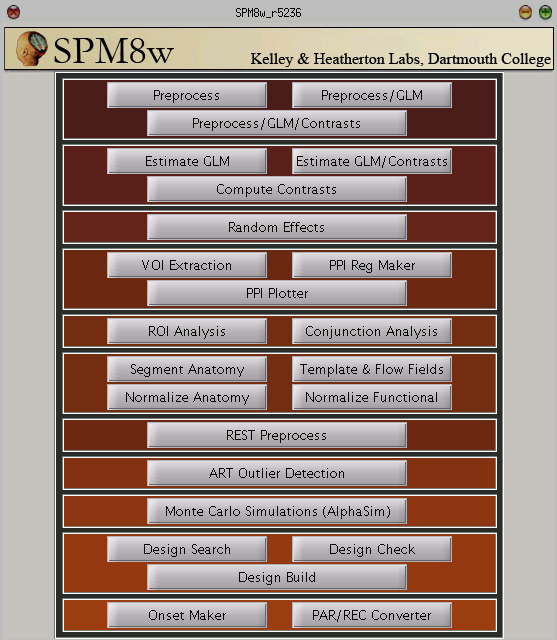
\includegraphics[keepaspectratio=true,scale=0.5]{./assets/4_spm8w}}
\end{minipage}

\subsection{Preprocessing}
SPM8w's command window output is designed to reduce clutter and suppress unimportant information and figures normally outputted by SPM while increasing the verbosity of important information (e.g. slice acquisition order, the precise onset filename, elapsed time for each stage, etc.). In addition, if onsets are already specified and a valid contrast file exists it is s possible to batch the entire 1st level analysis of a subject from preprocessing through to computing contrasts.

After selecting one of three preprocessing options in the menu, spm8w will prompt for subject selection and location of the parameter files. SPM8w relies heavily on regexp filters to only display the information needed for the current stage. Accordingly, a few simple naming rules must be followed. Subjects should be stored in the SUBJECTS directory and their name must follow the format ddsssddss (d = digit, s= character) (e.g. 12jan09aa)*. Parameter, CON, ROI, VOI, PPI and D files should be stored in the SCRIPTS directory and named appropriately (P\_H8TJAZZ.m; CON\_H8TJAZZ.m; ROI\_H8TJAZZ.m; VOI\_H8TJAZZ.m;). 

When selecting Preprocess from the menu, spm\_select will open in the SUBJECTS directory and display only directories whose name corresponds to the filter defined in spm8w\_defaults.m spm8w\_userdefaults.m (i.e. a regexp expression of form ddsssddss). As you make selections, they appear in the lower window and can be removed by clicking on them again. 

Next SPM8w will ask for the name of the parameters file, opening a selection window inside the SCRIPTS directory. Despite there being a number of files (P files, CON files, ROI files, etc.), spm\_select only displays the files whose name begins with P. Following this, preprocessing will begin, this generally takes anywhere from 25 minutes to over an hour. Progress information will be printed to the command window and a file containing all the command window output will be saved inside the subject’s directory (e.g. 27feb07aa\_diary.txt).


\subsection{Estimating a GLM}

Estimating the GLM proceeds in much the same way as preprocessing subjects. SPM8w will ask you to kindly select 1 or more subjects, specify the P file and afterwards GLM specification and estimation will begin. The only modifications here are:

The design matrix is saved to the file 27feb07aa\_model.pdf located in the subjects directory.
The location of bigmask.nii is explicitly referenced in the command window (this is for error checking in future versions where the choice of mask will be set in the P file, allowing us to try masks other than bigmask).  
The specific onsets that are going into the model will be referenced in the command window as they are loaded. This allows you to ensure that no conditions/onsets are missed due to typos or missing files. This include not only condition onsets, but associated \_dur and \_par files.
if p.outliers = 1, SPM8w will automatically add any outlier scans (specified in outliers\_run\#.txt created using ART Outlier Detection) as nuisance regressors to the GLM.  

\subsection{Computing Contrasts}
Computing contrasts works just as in the prior steps, requiring only the specification of which subject to run on and which P file to use. SPM8w allows the CON file to be specified within a study’s P file, obviating the need for selecting the CON file at this stage, however if the CON file was not specified in the parameters file, a spm\_select window will open asking that you select the appropriate CON file.

\subsection{Random Effects (RFX) Analysis}
Running an RFX analysis requires only that you select the directories for the conditions you want to run. SPM8w will open an spm\_select window in the study’s RFX directory. From there, select the RFX\_STUDYNAME directory in the left hand pane, this will navigate into that directory and then you can select the directories to run RFX analyses in by selecting them in the right pane. SPM8w will proceed to run one-sample t-tests on all the con image files in those directories. Alternatively you can select a study’s top-level RFX\_directory (i.e. RFX\_H8TJAZZ) and spm8w will run RFX on all the directories it finds inside.

\subsection{Regions of Interest (ROI) Analysis}
The ROI tool takes only an ROI parameters file as input. The rest of the analysis (parameter extraction, statistics) is guided entirely by the options set out in the ROI file. Below is an abbreviated output from an ROI analysis
ROI tool outputs two files: h8tjazz.txt, a tab delimited file containing ROI information and parameter estimates and h8tjazz\_stats.txt, containing the results of the statistics run on the parameter estimates. 
\subsection{VOI extraction}
Work in progress
\subsection{PPI Regressor Creation}
Work in progress
\newpage

%=Section 5
\section{Tools and Scripts}
\secttoc %Inserts a minitoc
\subsection{Design Search and Build}
Work in progress
\subsection{Conjunction Analysis}
The conjunction analysis option under spm8w will allow you to run a logical ‘AND’ conjunction analysis (see Valid Conjunction inference with the minimum statistic, Nichols, Brett, Andersson, Wager and Poline, 2005). This script is originally from Joe Moran and has been modified to allow for an unlimited number of inputs. The conjunction analysis option will ask you for the name of the output file (e.g. “conj\_h8tjazz”) the number of t-stat files to be used as inputs (e.g. 4) and will open an spm\_select window allowing you to navigate to your RFX directory and select the individual t-maps corresponding to the conditions to be tested for a conjunction. 
Once specified, spm8w\_conjunction will calculate the minimum t-value for each voxel and output a file (conj\_h8tjazz.img) with the minimum t-values. Interpretation of this spm requires that you view it thresholded at an appropriate level (e.g. same threshold you would use for any of the t-maps used as input). Voxels surviving thresholding can be interpreted as being conjointly active in each of the input t-maps.

\subsection{Monte Carlo Simulations with AFNI's AlphaSim}
The Monte Carlo Simulations option calls spm8w\_alphasim, which is a matlab wrapper for using AFNI’s AlphaSim program. AlphaSim will run a series of Monte Carlo simulations (defined in p.as\_iter) to determine a cluster size which when applied as an extent threshold will give a whole brain correction of p 0.05. Specifications for the simulation are set in the P file (see 1.4). In general, the threshold should be set to 0.001 (although 0.005 or 0.01 are often used) and the iterations should be 500 or more (1,000+ is good for publication). There is also the option to set the fast switch which speeds up the simulations by a factor of 2 at a small cost to accuracy. Additional inputs to spm8w\_alphasim are the mask delimiting the search volume and the estimated smoothness (FWHM in mm) of the GLM residuals. 

The extent threshold obtained from AlphaSim is largely determined by the size of the mask and the FWHM (in mm) of the residuals of the model. The mask can be any binary (bigmask, amygdala, fROI, etc.) however the mask must be in the same image space as the rest of the study, but can be in NIFTI format (no need to have masks in brik.hdr anymore). For instance, our original bigmask.img has a voxel size of 2x2x2 and needed to be resampled to 3x3x3. This mask comes with spm8w. In the future we might consider refining our mask to remove unnecessary elements (ventricles, cerebellum, possibly white matter).

Unfortunately SPM deletes the GLM residuals after estimation, however it calculates their smoothness and stores this information in the spm structure. For this reasons spm8w\_alphasim will ask for the SPM.mat file for the current analysis to specify the XYZ FWHM of the residuals for AlphaSim. It’s important to note that this FWHM value is not the same as the smoothing kernel used during preprocessing. For instance a fwhm smoothing of 8mm on our imaging data gives residuals whose smoothness is approximately 13 13 and 11.5, leading to an extent threshold of 58 contiguous voxels for whole brain correction. However this smoothness varies from RFX to RFX and it’s up to the user to decide if they want to recalculate the extent threshold for every RFX or take an average. As of SPM8 r.4010, the smoothness estimation was “improved” which has led to gross overestimation of smoothness when there are very few subjects (as in the example dataset 2012\_H8TJAZZ). Therefore I would recommend using the smoothness from a 1st level analysis as an estimate of the smoothness at the 2nd level. Not ideal, but the differences are slight. If you have sufficient subjects (n>10, perhaps), then the smoothness should be accurate. 
After selecting the appropriate SPM.mat, AlphaSim will run. This could take a couple of minutes depending on the number of iterations specified in the p.as\_iter field of your P file. Upon completion, the output of alphasim will be saved to the filename specified in p.as\_fname (e.g.‘as\_h8tjazz.txt’) and spm8w\_alphasim will print out the extent threshold required for a whole brain correction at the specified threshold. 

\subsection{Onset Maker}
Onset maker is a simple script to make it easier to create onset files for use with spm8w. Onset maker takes as input an appropriately formatted csv file (such as one exported from excel, see below for an example) and will ouput condition.txt files, condition\_parametric.txt files and subject\_condition\_duration.txt files. In addition, Onset Maker will replace any N/A or NaN duration values with the within condition mean duration. For instance, if your durations are subject RTs and the subject failed to respond to a number of items, those items will be replaced with the mean RT for that condition.

Onset Maker is not set up to create subject specific condition onsets or subject specific 
parametric onsets, but could potentially be modified to do so in the future if needs be (alternatively you can hijack the duration specification for subject specific onsets or parametrics and just rename the subjid\_condition\_dur.txt files to subjid\_condition.txt files or subjid\_condition\_par1.txt files). 
Onset maker can be called either from spm8w or directly from the command window (e.g. spm8w\_onsmaker() or spm8w\_onsmaker(‘onsets.csv’)). Onset maker will attempt to open a spm\_select window in your ONSETS directory and ask you to specify the csv file containing onset specifications, you can however store your csv anywhere you’d like and if there is no local ONSETS directory spm\_select will open in place. Onset maker will output a series of textfiles based on the specifications in the onsets.xls file. 
\newpage

%=Section 6
\section{Examples}
\secttoc %Inserts a minitoc
\subsection{Event-related with parametric regressors}
\subsection{Event-related modeling reaction times}
\subsection{Block Design}
\subsection{Mixed Design(state-item)}
\subsection{PPI Analysis}
\newpage

%=Section 7
\section{Appendix}
\secttoc %Inserts a minitoc
\subsection{Contributors}
A number of people have knowingly, or unknowingly, contributed code to SPM2w and SPM8w over the years. Joe Moran in particular has been lied, cheated to and stolen from on numerous occasions (always with permission). In addition, some code for state-item analysis is derived from scripts shared by Gagan Wig. Calculation of slice-wise noise is derived from Antonia Hamilton's slice noise analysis scripts. Finally, spm8w\_art.m uses an older version of art\_detect by Sue Gabrieli and others (provided as part of SPM8w with permission from the author). 

The origins of the original code from which SPM8w derives is unknown. Around 2005, our labs switched to a set of SPM2 scripts cobbled together from our prior SPM99 scripts and some unknown source who may or may not have been Antonia Hamilton. SPM2w was initially created from these scripts simply in order to have an lazier way of batchign subjects. The 'w', which stands for 'wicked', was added so that both sets of scripts could co-exist on the same path. 

Over time, SPM2w was modified and extended and eventually ported to SPM8 which resulted in a large re-write of the code and further functionality. The move to SPM8 brought along a host of new functions (from Joe Moran: outlier detection, conjunction analysis and spherical ROI creation, among others). Addition tools from DDW include the roi and voi tools, SNR analysis, dartel normalization among other things. For the gory details check the change log below. 

\subsection{spm8w change log}
\noindent
\textbf{April 2010 - SPM8w\_3684:}
\begin{itemize}
	\item Spm8w.m: moved redundant code to functions
	\item Spm8w.m: rewrote error handling routine so that crashes return user to root directory and display last error message.
	\item Spm8w.m: RFX analysis will now determine if user selected top level RFX directory and run RFX in all subdirectories (1 level deep). 
	\item Spm8w.m: Added colorful shiny gui instead of pulldown.
	\item Spm8w\_userdefaults.m: Some defaults for subject name filtering and all welcome and error messages can be edited. Spm8w\_userdefaults.m must live in user’s matlab path. If none exists, spm8w will use its own defaults.
	\item Spm8w\_preprocess.m: cleaned up code a bit, added calls to spm8w\_userdefaults and \newline spm8w\_defaults.m
	\item Spm8w\_compute.m: Fixed effects of interest so that it no longer includes nuisance regressors.
	\item Spm8w\_compute.m: re-wrote large portions of spm8w\_compute’s logic and removed \newline spm8w\_mk\_regressors.m (it’s now a function inside spm8w\_compute and called \newline make\_nuissance). The idea now is that make\_nuissance handles nuisance regressors and we no longer trick it into making block regressors for sate-item. That step is now performed during design specification. Also added sections to accommodate regression only designs (to be added in the future). 
	\item P and CON files updated (some fields removed, added p.slicetime and p.reg\_cond (for regression only designs, not supported yet). 
	\item Paths now do a spm/spm8w version check so user can be sure of what versions are loaded.
\end{itemize}
\noindent
\textbf{August 2010 - SPM8w\_4010:}
\begin{itemize}
	\item Spm8w.m: SPM8r4010 invalidates calls to spm\_defaults, edited to reflect the new way of calling defaults (i.e.: spm(‘defaults’,’fmri’)).
	\item Some scripts outputs have been made more verbose. In particular, GLM computation will now tell you exactly what onset files (both conditions, durations and parametric files) it’s using as it loads them so there’s no more mystery as to what’s going into the GLM. 
	\item Finalized inclusion of regressor only designs (i.e. spm8w\_compute.m). Spm8w can now include user regressor that will not be convolved with the HRF. These must be in an onsets directory and equal the number of TRs in the study. 
	\item Added new script: spm8w\_nifticonverter - for converting backed up RAW par/rec data to nifti format and placing it in appropriate directory for a study, type \newline ‘help spm8w\_nifticonverter’ for info.
	\item Added new script: spm8w\_voitoool – general purpose script for extracting timeseries, creating PPI regressor and plotting PPIs. Type ‘help spm8w\_voitool’ for info.
	\item Spm8w\_onsmaker.m has been modified so that input must be in csv (xlsread was giving too many errors due to poor implementation on unix). 
	\item Spm8w\_roitool.m has been modified to allow for multiple correlations (it will iterate \newline through any input correlation files) in the basic stats section.
	\item Spm8w\_compute.m has been modified to allow runs to be modeled separately \newline (p.include\_run must be in P file). 
	\item Added various commands to all scripts to clean up the variable space. 
	\item Added mni2tal and tal2mni to tools path (finally).
\end{itemize}
\noindent
\textbf{November 2011 - SPM8w\_4290:}
\begin{itemize}
	\item Tweaked realignment (made spm8w\_realign.m more verbose) added option to do 2 pass realign to mean in P file. 
	\item Added option to specify write out parameters for reslicing/warping (p.voxsize, \newline p.boundbox, p.wrap, p.interp). These have been set to the SPM8 defaults (spm2 defaults that we used to use are in comments). See “How the revisions affect the statistics” for evidence that this has a negligible effect.
	\item Fixed bug where realignment parameters are never plotted due to SPM8 using findwin instead of getwin.
	\item Cleaned up figure printing. Figures during prepro are appended to a .ps file which gets converted to a pdf at final stages using ps2pdf.m (included with spm8w). Should help make this more cross-platform since it uses matlab’s internal ghostscript. Spm8w\_compute, dumps straight to pdf using the GLM directory name for naming. 
	\item Added early version of design search and build to menu. Still needs work. 
	\item Changed the behavior of spm8w\_compute to delete prior GLMs before overwriting (otherwise requires user intervention due to spm warning). GLM calc is short and normally we always want to overwrite. 
	\item Added basic orthogonality checking to design matrix. Spm8w\_compute.m now puts a correlation matrix color coded for negative and positive correlations between regressors.
	\item Changed formula for calculating regressors of no interest to strcmp or else is fails when user creates a regressor only design and uses the letter r in the name of the regressor.
	\item spm8w\_preprocess now always deletes prior preprocessing if found. In fact it clear the folder except for raw bold files. 
	\item Added option to use 3dDespike and perform a slice noise analysis in prprocessing
	\item Cleaned up code for figure printing throughout (figures are now always hidden except at GLM). 
	\item Added code to do a slice-wise noise analysis during preprocessing.
	\item Small bug fixes having to do with catching non-standard preprocessing.
\end{itemize}
\noindent
\textbf{March 2012 - SPM8w\_4667}
\begin{itemize}
	\item First pass at making spm8w cross-platform
	\item Updated a few things in spm8w\_roitool.m
	\item Added support for new tool spm8w\_art.m which will save outlier volumes in the subject FUNCTIONAL dir for incorporating in the model (p.outlier =1 in the P file).
	\item Cleaned up spm8w\_compute.m (mk\_nuissance). Changed order, concat regressors (rather than guess and fail) and added support for outliers. 
	\item Added p.polyord to the P file. spm8w\_compute will now include polynomial trends to account for drift and other LF noise. A polynomial order of 1 is identical to the linear trend regressor we’ve always used. Higher order polynomials will model different trends (quadratic, cubic) which is useful for longer runs. 
	\item Cleaned up spm8w\_compute.m (mk\_nuissance) again to get rid of redundancies and check if exist onset files for better error checking. 
	\item More fixes to spm8w\_compute. Setting p.outliers to 1 will now not crash if there are no outliers. This way you can add outliers if they exist, and if not, proceed anyway.
	\item New script. spm8w\_renamer. For massive renaming of files. Work in progress.
\end{itemize}
\noindent
\textbf{March 2013 - SPM8w\_5236}
\begin{itemize}
	\item Added VBM8 toolbox (useful for segmentation and DARTEL normalization).
	\item DARTEL based normalization integrated into our preprocessing workflow. 
	\item Within-trial orhtogonalization is no longer disabled by default but rather \newline spm\_fMRI\_design.m now checks a global variable (disable\_orth set by p.disable\_orth) to see if within-trial orthogonalization should be disbaled
	\item SPM8w\_compute.m now supports GLMs based on DARTEL or VBM8 DARTEL normalization and additionally supports running GLMs with different number of TRs per run. 
	\item Major overhaul to spm8w\_roitool.m: support for roi specifications and variable specifications from excel files based on subjID to excel ID matching (much safer than the previous alphabetical sort and pray it matches method). Re-wrote statistics functions to improve presentation and include between subject t-tests.  
	\item Major overhaul to spm8w\_nifticonverter.m: Uses new directory conventions and will uncompress and convert raw\_subjID.tar.gz files using r2a\_gui, parsing the output into the subID/NIFTI directory. 
	\item Major overhaul to spm8w\_voitool.m: Cleaned code and fixed local maxima search. Now properly searches for best nearest local maxima within a distance from the target voxel (rather than simply take the nearest suprathreshold voxel). 
	\item New tool: spm8w\_updatechk.m compares the revision of SPM8 files to their modified spm8w counterparts. Useful when SPM8 is updated to a new revision to see if SPM8w modified versions need updating.
	\item New tool: spm8w\_getavgsmooth.m Calculates and returns the mean FWHM of the 1st level GLMs across subjects selected by the user for a provided P file. This function is called by spm8w\_alphasim.m to determine the FWHM to use for monte-carlo simulations. 
	\item New tool: spm8w\_mriqa.m Generates a PDF of multiple slices of each subjects anatomical MRI for fast QA (useful prior to MRI anatomical segmentation). 
	\item New tool: spm8w\_rawtar.m Matlab version of our old linux rawtar command. Compresses tar archives of raw PAR/REC directories (in truth it should work on any directory). This allows Windows users to use rawtar.  
	\item New tool: spm8w\_dartel.m Controls all aspects of DARTEL normalization.
	\item New tool: spm8w\_tester.m Simple testing script which will run the example dataset \newline through most analyses. Should be the first thing people run after a fresh install to make sure everything works. 
	\item New tools: statsw\_zscore.m Simple z-score implementation to use in place of the stats toolbox code (since we sometimes run out of stats toolbox licenses depending on concurrent use). 
	\item First attempt at adding aspects of resting state preprocessing to our workflow. Work in progress.	
\end{itemize}

\subsection{Changes from spm2 to spm8w}
\textit{note: the changes are getting to be too many to mention. So I'm not going to update this section anymore. Most people haven't touched spm2/spm2w batch scripts in years -November 2011}

\noindent
\textbf{Changes:}
\begin{itemize}
	\item New standard study directory structure (i.e. /SCRIPTS, /ONSETS, /RFX, /SUBJECTS, /SNR, /ROI, /PS)
	\item Built-in batch loop (e.g. can run on < 4 subjects) and more flexible options (e.g. prepro-glm-contrasts all in one go).
	\item Onsets can have custom names and are stored in a common ONSETS directory.
	\item Option to delete intermediary files (e.g. abold, uabold, etc.)
	\item Moved some critical variables to the parameter file so that they are less hidden.
	\item Scripts print out  more detailed information in the command window and save a log of the command window 
	\item Added filtering to spm\_select to speed up selection (P, CON, ROI and subject filters) 
	\item Tweaked command window output to reduce visual clutter. Figures now only spawn when needed for postscript printing.
	\item Durations can be specified in seconds as well as TRs (see p.durtime)
\end{itemize}
\noindent
\textbf{Default Changes:}
\begin{itemize}
	\item Bounding box is slightly different than SPM2 to fix problem with default origin being off after normalization.
	\item Realignment quality changed to spm8 default of 0.9 (spm2 was 0.75).
	\item Unwarping basis function changed from [10 10] to [12 12]
	\item Normalization interpolation set to 7 (spm8 default is 1, spm2 default was 7 ***I think, hard to tell due to change from text to number between spm2 and spm8)
	\item Normalization write wrap is set to spm2 default of [0 1 0] (spm8 default is [0 0 0]).
	\item Added the RFX design structure to the spm8w\_do\_rfx rather than in a separate .mat file.
	\item Spm8w will always clear a previous RFX before running (to prevent file collisions and spm\_select from grabbing stray con files).
\end{itemize}
\noindent
\textbf{Additions:}
\begin{itemize}
	\item State-item designs are specified in the parameters file and no longer require custom hacks
	\item SNR calculation is part of the preprocessing stream and the SNR figures will be printed to prepro.ps
	\item Option to demean task regressors which will make spm2/5/8 orthogonality checks equivalent to spm99.
	\item Contrasts script pads nuisance variables with zeros (from JM)
	\item New flexible ROI tool for most excellent parameter estimate extraction!
	\item New wrapper for AFNI’s AlphaSim, grabs residual FWHM from the spm.mat for a given analysis.
	\item Logical conjunction script based on JM’s conjunction script.
\end{itemize}
\noindent
\textbf{Fixes:}
\begin{itemize}
	\item Crash when slice-timing is turned off (hardcoding issue)
	\item Increased the max contrast length limit (previously it was set to 99 regressors)
	\item Order of slices for Philips Interleaved sequences is now correctly specified.
	\item Fixed figure display for when number of runs are greater than 6.
	\item Maximum number of parametric regressors is now 3 (instead of 1)
	\item Duration and para can be subject specific (e.g. 02jun01aa\_dur.txt) but condition regressors can remain global.
	\item SPM.xCon is manually set (spm8 no longer specifies this in the spm structure).
	\item Can specify a HPF or Autocorrelation (probably only valid if you have a single run)
\end{itemize}

\subsection{Upgrading SPM8 revions}
One of the advantages of SPM8w is the way it outputs progress and diagnostic information to the command window and generates a set of PDF files from SPM's output for Q.A. purposes. This is also a downside as it means that a number of core SPM8 files have been duplicated and modified (i.e. SPM8w calls spm8w\_normalise.m instead of spm\_normalise.m). The fallout of this practice is that every new SPM8 revision requires that we duplicate the updated files and re-implement our modifications at the appropriate lines. The exact files that need to be modified are described below.

Whenever possible SPM8w leaves the core SPM8 files intact and uses renamed versions of these files (e.g. spm8w\_normalize.m). There is one exception to this rule, the file \newline spm\_fMRI\_design.m which are is tightly integrated in SPM to call a renamed version.

Not all SPM8 files are revised at every SPM8 revision, therefore it will often be the case that many of the modified SPM8 files that ship with SPM8w won't require any modification.  An easy way to check is to use the built in SPM8w revision checker (spm8w\_updatechk.m) to see if the scripts modified by SPM8w have been changed with the latest SPM8 update. Simply call spm8w\_updatechk from the matlab command prompt. 

\vspace{\baselineskip}
\noindent
\textbf{Currently SPM8w (r5236) calls renamed versions of the following files:}
\begin{itemize}
	\item spm8w\_realign.m  --- replaces calls to spm\_realign.m [revision 4152]
Edits involve disabling spm graphics and making output more verbose. Altering line 454 to spawn a figure window (otherwise realignment never gets plotted). Tweaked figure to add more space for filenames
	\item spm8w\_slice\_timing.m --- replaces calls to spm\_slice\_timing.m [revision 4310]
Edits involve disabling spm graphics .
	\item spm8w\_uw\_estimate.m --- replaces calls to spm\_uw\_estimate.m [revision 4310]
Edits involve disabling spm graphics.
	\item spm8w\_normalise.m --- replaces calls to spm\_normalise.m [revision 4621]
Edits involve disabling spm graphics. In spm 4290 defaults changed (cutoff is now 24 instead of 30, reg is 1 instead of 0.1) 
	\item spm8w\_normalise\_disp.m  --- replaces calls to spm\_normalise\_disp.m [revision 1143]
Edits involve disabling spm graphics on lines. Changing FindWin calls to GetWin
	\item spm8w\_preproc\_run.m  --- replaces calls to spm\_preproc\_run.m [revision 4667]
Edits involve disabling spm graphics and making output more verbose
	\item spm8w\_maff8.m  --- replaces calls to spm\_maff8.m [revision 4152]
Edits involve disabling spm graphics and making output more verbose
	\item spm8w\_preproc8.m  --- replaces calls to spm\_preproc8.m [revision 4148]
Edits involve disabling spm graphics and making output more verbose
	\item spm8w\_preproc\_write8.m  --- replaces calls to spm\_preproc\_write8.m [revision 4337]
Edits involve disabling spm graphics and making output more verbose
	\item spm8w\_dartel\_norm\_fun.m  --- replaces calls to spm\_dartel\_norm\_fun.m [revision 4194]
Edits involve disabling spm graphics, making output more verbose and accepting normtok (i.e., DARTEL or VBM8). 
	\item spm8w\_dartel\_template.m  --- replaces calls to spm\_dartel\_template.m [revision 4064]
Edits involve disabling spm graphics and making output more verbose
	\item spm8w\_dartel\_warp.m  --- replaces calls to spm\_dartel\_warp.m [revision 4064]
Edits involve disabling spm graphics and making output more verbose and listing current iteration.
\end{itemize}

\noindent
\textbf{And the following core SPM8 files are modified:}
\begin{itemize}
	\item spm\_fMRI\_design.m  [revision 4185] --- Line: 277-290 Within trial type (e.g. condition) orthogonalization is controlled by checking the global variable disable\_orth (set from p.disable\_orth in the P file). This allows the P file to control whether p.disable\_orth is on or off rather than disabling for everyone. 
\end{itemize}

Importantly for prior users of SPM8w, we no longer alter the spm\_flip\_analyze\_images.m file since it is only for files with missing transformation fields in the header, such as occurs when converting from analyze to NIFTI. With true NIFTI files, this setting has no effect. This is critically important as anyone who uses an older analyse file (even if in NIFTI format) may find themselves with wrong handed images and significant egg on face when they realize it.

\vspace{\baselineskip}
When upgrading to a new SPM8 revision, it is probably a good idea to conserve the extra files that we added to the canonical directory (i.e. copy them from the old SPM8 revision into the new revision's canonical directory). These can also be found in the canonical.7z archive in the ADDITIONAL\_FILES directory that ships with SPM8w. 
\begin{itemize}
	\item aal.nii --- AAL brain
	\item brodmann.nii --- Brodmann area map
	\item ch2.nii --- Higher resolution colin brain (single subject T1)
	\item ch2bet.nii --- Higher resolution colin brain with skull extracted
	\item ch2better.nii --- Better skull extraction?
\end{itemize}

\subsection{How new revisions change spm statistics}
In general, SPM8 and SPM8w revisions should have negligible effects on the statistical maps. The following keeps track of a few coordinates per update in order to ensure that changes to default parameters, code revisions and platform changes have negligible effects. NB: As of SPM8w r5236, the example data has changed and the 27feb07aa subject is no longer provided. I will, however, continue to analyze these same coordinates with that subject through each update and put the results here. 

\begin{center}
\begin{tabular}{ll}
	\hline
	\multicolumn{2}{l}{\textbf{SPM8 r3408 -- SPM8w v0 (January, 2010) - Matlab 7.4}}\\
	\hline
	Subject: 27feb07aa & Map:spmT\_0002.img\\
	\hline
	Coordinate: -36,-78,-39 (global maxima) & T-value: 21.88\\
	Coordinate: -6,-9,51 (dACC) & T-value: 5.75\\
	Coordinate: -60,-15,51 (Left Motor) & T-value: 11.68\\
	\hline \\
\end{tabular}

\begin{tabular}{ll}
	\hline
	\multicolumn{2}{l}{\textbf{SPM8 r3684 -- SPM8w v3684 (April, 2010) - Matlab 7.4}}\\
	\hline
	Subject: 27feb07aa & Map:spmT\_0002.img\\
	\hline
	Coordinate: -36,-78,-39 (global maxima) & T-value: 22.74\\
	Coordinate: -6,-9,51 (dACC) & T-value: 5.52\\
	Coordinate: -60,-15,51 (Left Motor) & T-value: 12.07\\
	\hline \\
\end{tabular}

\begin{tabular}{ll}
	\hline
	\multicolumn{2}{l}{\textbf{SPM8 r4010 -- SPM8w v4010 (August, 2010) - Matlab 7.4}}\\
	\hline
	Subject: 27feb07aa & Map:spmT\_0002.img\\
	\hline
	Coordinate: -36,-78,-39 (global maxima) & T-value: 22.62\\
	Coordinate: -6,-9,51 (dACC) & T-value: 5.50\\
	Coordinate: -60,-15,51 (Left Motor) & T-value: 11.99\\
	\hline \\
\end{tabular}

\begin{tabular}{ll}
	\hline
	\multicolumn{2}{l}{\textbf{SPM8 r4290 -- SPM8w v4290 (November, 2011) - Matlab 7.4}}\\
	\multicolumn{2}{l}{\textit{Also tested Matlab 7.11 and same results. Upgrade matlab with impunity!}}\\
	\hline
	Subject: 27feb07aa & Map:spmT\_0002.img\\
	\hline
	Coordinate: -36,-78,-39 (global maxima) & T-value: 22.73\\
	Coordinate: -6,-9,51 (dACC) & T-value: 5.43\\
	Coordinate: -60,-15,51 (Left Motor) & T-value: 11.94\\
	\hline \\
\end{tabular}

\begin{tabular}{ll}
	\hline
	\multicolumn{2}{l}{\textbf{SPM8 r4290 -- SPM8w v4290 (November, 2011) - Matlab 7.4}}\\
	\multicolumn{2}{l}{\textit{With new 4290 defaults: RTM=0,WRAP=[0 0 0],INTERP\_R=7, INTERP\_W=7}}\\
	\hline
	Subject: 27feb07aa & Map:spmT\_0002.img\\
	\hline
	Coordinate: -36,-78,-39 (global maxima) & T-value: 22.90\\
	Coordinate: -6,-9,51 (dACC) & T-value: 5.50\\
	Coordinate: -60,-15,51 (Left Motor) & T-value: 11.96\\
	\hline \\
\end{tabular}

\begin{tabular}{ll}
	\hline
	\multicolumn{2}{l}{\textbf{SPM8 r4667 -- SPM8w v4667 (March, 2012) - Matlab 7.4}}\\
	\hline
	Subject: 27feb07aa & Map:spmT\_0002.img\\
	\hline
	Coordinate: -36,-78,-39 (global maxima) & T-value: 22.90\\
	Coordinate: -6,-9,51 (dACC) & T-value: 5.50\\
	Coordinate: -60,-15,51 (Left Motor) & T-value: 11.96\\
	\hline \\
\end{tabular}

\begin{tabular}{ll}
	\hline
	\multicolumn{2}{l}{\textbf{SPM8 r4667 -- SPM8w v4667 (March, 2012) - Matlab 7.11(2010b)}}\\
	\multicolumn{2}{l}{\textit{Run entirely in Microsoft Windows on a PC}}\\
	\hline
	Subject: 27feb07aa & Map:spmT\_0002.img \\
	\hline
	Coordinate: -36,-78,-39 (global maxima) & T-value: 22.90\\
	Coordinate: -6,-9,51 (dACC) & T-value: 5.50\\
	Coordinate: -60,-15,51 (Left Motor) & T-value: 11.96\\
	\hline \\
\end{tabular}

\begin{tabular}{ll}
	\hline
	\multicolumn{2}{l}{\textbf{SPM8 r4667 -- SPM8w v4667 (March, 2012) - Matlab 7.11(2010b)}}\\
	\multicolumn{2}{l}{\textit{Run entirely in Microsoft Windows on a PC}}\\
	\hline
	Subject: 27feb07aa & Map:spmT\_0002.img \\
	\hline
	Coordinate: -36,-78,-39 (global maxima) & T-value: 22.90\\
	Coordinate: -6,-9,51 (dACC) & T-value: 5.50\\
	Coordinate: -60,-15,51 (Left Motor) & T-value: 11.96\\
	\hline \\
\end{tabular}

\begin{tabular}{ll}
	\hline
	\multicolumn{2}{l}{\textbf{SPM8 r5236 -- SPM8w v5236 (April, 2013) - Matlab 8.0 (2012)}}\\
	\multicolumn{2}{l}{\textit{Run entirely in Microsoft Windows on a PC}}\\
	\hline
	Subject: 27feb07aa & Map:spmT\_0002.img \\
	\hline
	Coordinate: -36,-78,-39 (global maxima) & T-value: 22.63\\
	Coordinate: -6,-9,51 (dACC) & T-value: 5.66\\
	Coordinate: -60,-15,51 (Left Motor) & T-value: 11.36\\
	\hline \\
\end{tabular}

\end{center}
 
\newpage

%=Section 8
\section{FAQ}
\secttoc %Inserts a minitoc
\subsection{What are my options for dealing with motion?}
There are four ways to deal with motion within the context of what is available in SPM8w:
\begin{enumerate}
	\item Nothing but realignment. (p.realign = 1)
	\item Unwarp to correct for Movement by Susceptibility interactions (p.unwarp = 1) \newline(see: \url{http://www.fil.ion.ucl.ac.uk/spm/toolbox/unwarp})
	\item Include the realignment parameters as motion covariates in the GLM (p.move = 1)
	\item Use Art Outlier Detection to remove (i.e., censor) time points with large motion. Often you also want to grab 1 or 2 timepoints proceeding and following the motion spike. (p.outliers = 1).
\end{enumerate}
Unwarping and including realignment parameters as covariates is most certainly overkill as the covariates and unwarping are redundant. Generally, in cases of reasonable motion, it may be sufficient to perform unwarping and not include the realignment parameters. This is because the realignment parameters can have a detrimental effect on sensitivity if movement correlates with the task (even if small). See Johnstone's paper on the pitfalls of always including realignment parameters (\url{http://www.keck.waisman.wisc.edu/~tjohnstone/Johnstone_HBM_Oct_2006.pdf}). That being said, we still typically do both (unwarp and include realignment parameters in the GLM). 

\subsection{How should I filter or detrend my data for low frequency noise?}
FMRI data typically contains a high degree of low-frequency "noise". Sources of this noise vary from physiological signals (e.g., respiration) to scanner signal drift. Different analysis packages have implemented a number of methods for "filtering" out this LF noise. Some packages employ temporal filtering prior to GLM modeling, effectively creating a new dataset in which LF noise has been removed. However, most packages these days appear to model the LF noise at the GLM phase. SPM used to include a series of cosine regressors in the model (discreet cosine matrix or DCT) which capture variance associated with low frequency components of the timeseries. Later versions instead filtered the entire design matrix through the DCT, effectively resulting in a model that will filter out low frequencies, but without losing any degrees of freedom due to the inclusion of additional regressors. AFNI, on the other hand, typically accounts for low frequency trends in the data by including a series of polynomial regressors in the GLM. The simplest of these (-polort 1) is a constant plus a linear trend regressors. 

Within the context of SPM8w, we've typically only included a constant and linear trend term (per session) rather than use SPM's DCT method. The primary reason for this is that, unlike traditional SPM analyses, we concatenate event vectors into a single regressor per condition (i.e., we concatenate runs). It is unclear, at this time, if the DCT method used by SPM is valid when concatenating runs (however at a MGH workshop Dan Gittelman suggested this wasn't a big deal and it was fine to use SPM's traditional high pass filter on concatenated data). With SPM8w, we follow the same conceptual method as the AFNI folk by using a 1st order polynomial to model low frequency trends in the data (i.e. a linear trend regressor per session).

With the latest SPM8w revision, we've added the option to include more polynomials. \newline Specifically, p.polyord specifies the order of the polynomials to include in the design. Setting p.polyord = 0 models only the session mean, and does not model trends at all (not recommended). p.polyord = 1 is identical to including the linear term in previous SPM8w versions. p.polyord = 2 or 3 adds 2nd and/or 3rd order polynomials to the model (i.e., quadratic and cubic trends). Increasing the number of polynomials beyond this is allowed, but it generally not necessary(see \url{http://www.sciencedirect.com/science/article/pii/S1053811902910530}). 

Here is the timeseries and power spectra for one voxel (MNI: -21,-6,-21) of one run of 268 TRs, 3 Conditions + 2 Instruction Conditions (on/off cues) and 6 motion covariates (made with spm8w\_timeplot.m). The opaque band in the Frequency domain graphs highlights the portion of the frequency spectrum typically filtered out by using a 128second filter (SPM's default). At least for this voxel, there’s not much power in the LF range to worry about, even without filtering.

\vspace{\baselineskip}
\noindent
Raw data (prior to GLM, mean centered only):

%Insert image using minipage
\vspace{\baselineskip}
\noindent%
\begin{minipage}{\linewidth}
\makebox[\linewidth]{%
  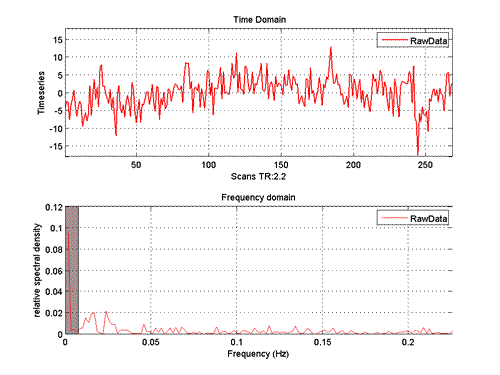
\includegraphics[keepaspectratio=true,scale=0.5]{./assets/8_timeplot1}}
\end{minipage}

\vspace{\baselineskip}
\noindent
This figure shows the power spectrum for the same timeseries with linear trend removal:

%Insert image using minipage
\vspace{\baselineskip}
\noindent%
\begin{minipage}{\linewidth}
\makebox[\linewidth]{%
  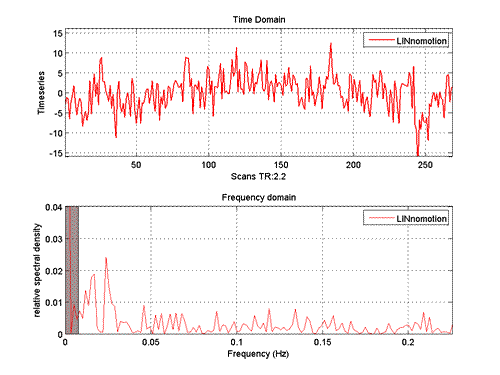
\includegraphics[keepaspectratio=true,scale=0.5]{./assets/8_timeplot2}}
\end{minipage}

\vspace{\baselineskip}
\noindent
And here’s the same timeseries with p.polyord = 2. LF noise is almost as good as SPM's HPF and the time series itself is flatter. It seems that p.polyord = 2 is best. One could go to p.polyord =3, but in my tests this did not improve above modeling linear and quadratic trends. It may matter with longer runs.

%Insert image using minipage
\vspace{\baselineskip}
\noindent%
\begin{minipage}{\linewidth}
\makebox[\linewidth]{%
  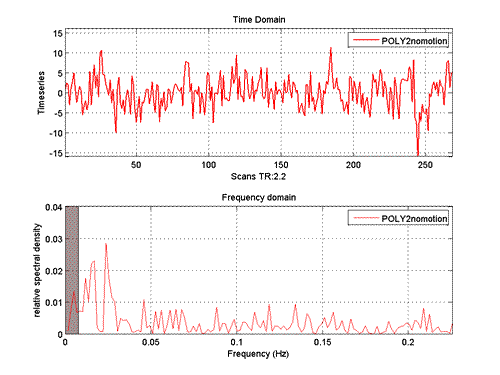
\includegraphics[keepaspectratio=true,scale=0.5]{./assets/8_timeplot3}}
\end{minipage}
\newpage

\end{document}